\documentclass[aspectratio=169]{beamer}
\usepackage{color,amsmath}
\usepackage{subfigure}
\usepackage{booktabs}
\usepackage{framed}
\usepackage{comment}

\usepackage{ulem}

\usepackage{hyperref}
\hypersetup{
    colorlinks=true,
    linkcolor=blue,
    filecolor=magenta,      
    urlcolor=cyan,
}

%%%%%%%%%%%%%%%%%%%%%%%%%%
\title[]{[Survey research in the digital age]\textcolor{gray}{, [Probability and non-probability sampling], [Computer-administered interviews], [Combining surveys and big data], [Additions and extensions]}}
\author[]{Matthew J. Salganik\\Department of Sociology\\Princeton University}
\date[]{%Summer Institutes in Computational Social Science\\2020
%\vfill
%\begin{flushleft}
%{\scriptsize
%The Summer Institutes in Computational Social Science is supported by grants from the Russell Sage Foundation and the Alfred P. Sloan Foundation.}
%\end{flushleft}
\begin{flushright}
\vfill

\includegraphics[width=0.1\textwidth]{figures/cc-by.png}
\end{flushright}
}
\begin{document}
%%%%%%%%%%%%%%%%%%%%%%%%%%
\frame{\titlepage}
%%%%%%%%%%%%%%%%%%%%%%%%%%
\begin{frame}

\begin{columns}
\begin{column}{.40\textwidth}
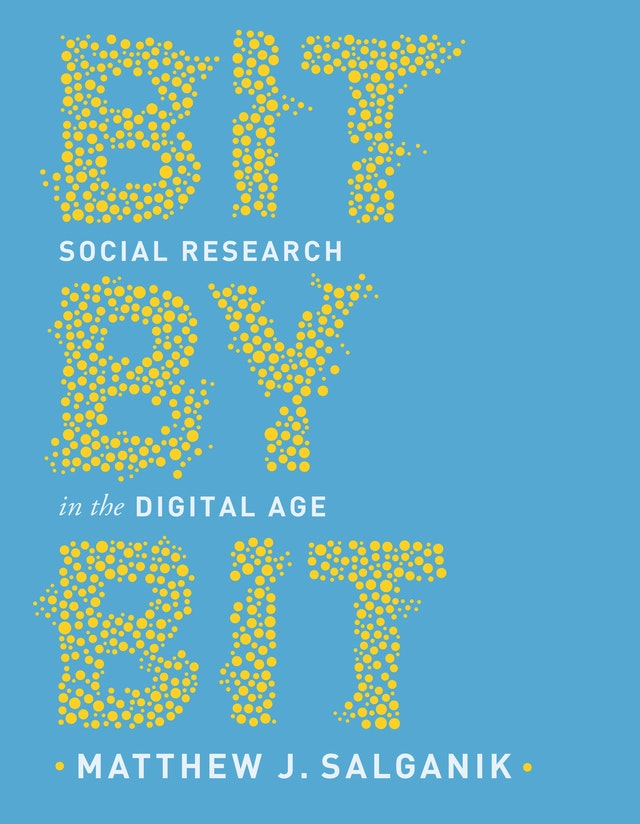
\includegraphics[width=\textwidth]{figures/salganik_bit_2018_cover}
\end{column}%

\hfill%

\begin{column}{.60\textwidth}
1) Introduction \\
2) Observing behavior \\
\textcolor{blue}{3) Asking questions} \\
4) Running experiments \\
5) Mass collaboration \\
6) Ethics \\
7) The future \\
\end{column}%
\end{columns}

\end{frame}
%%%%%%%%%%%%%%%%%%%%%%%%%%
\begin{frame}

\begin{center}
\begin{tabular}{ccc}
\onslide<1-3>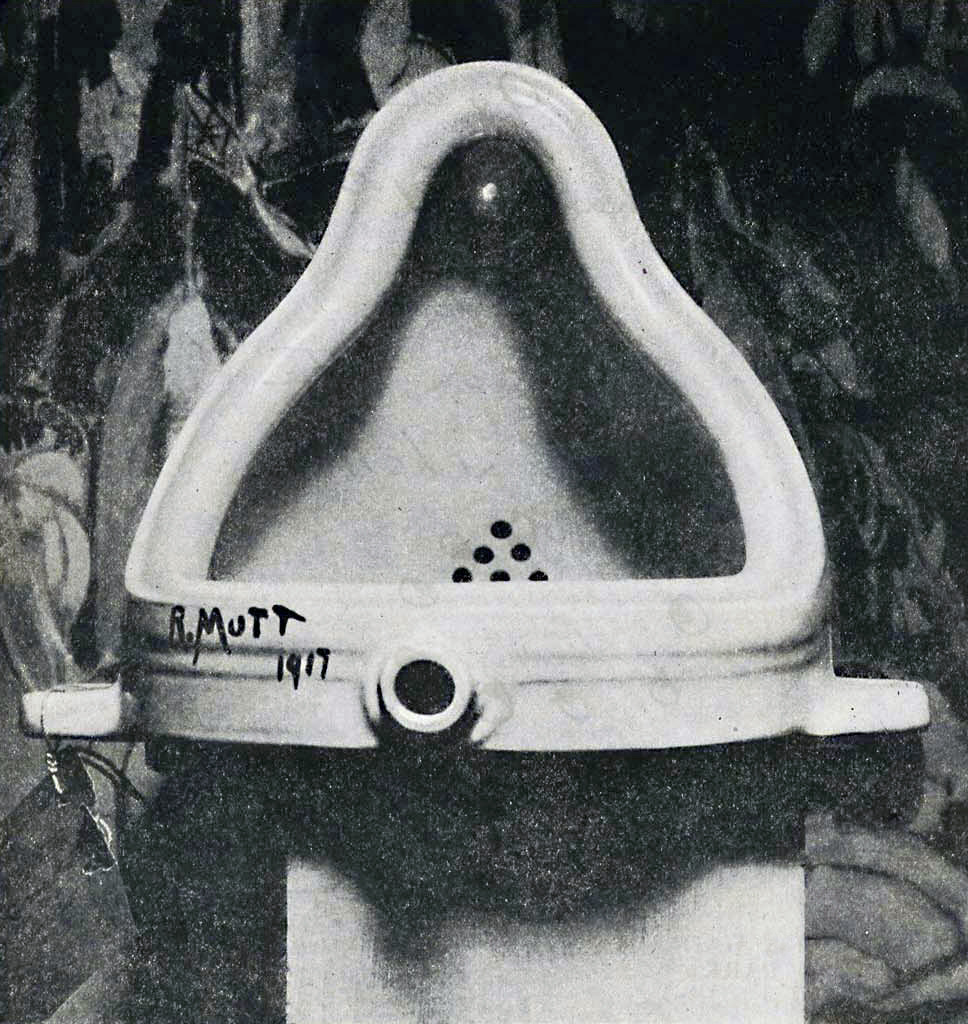
\includegraphics[width=0.30\textwidth]{figures/duchamp_fountain} & \phantom{12345} & \onslide<2-3>{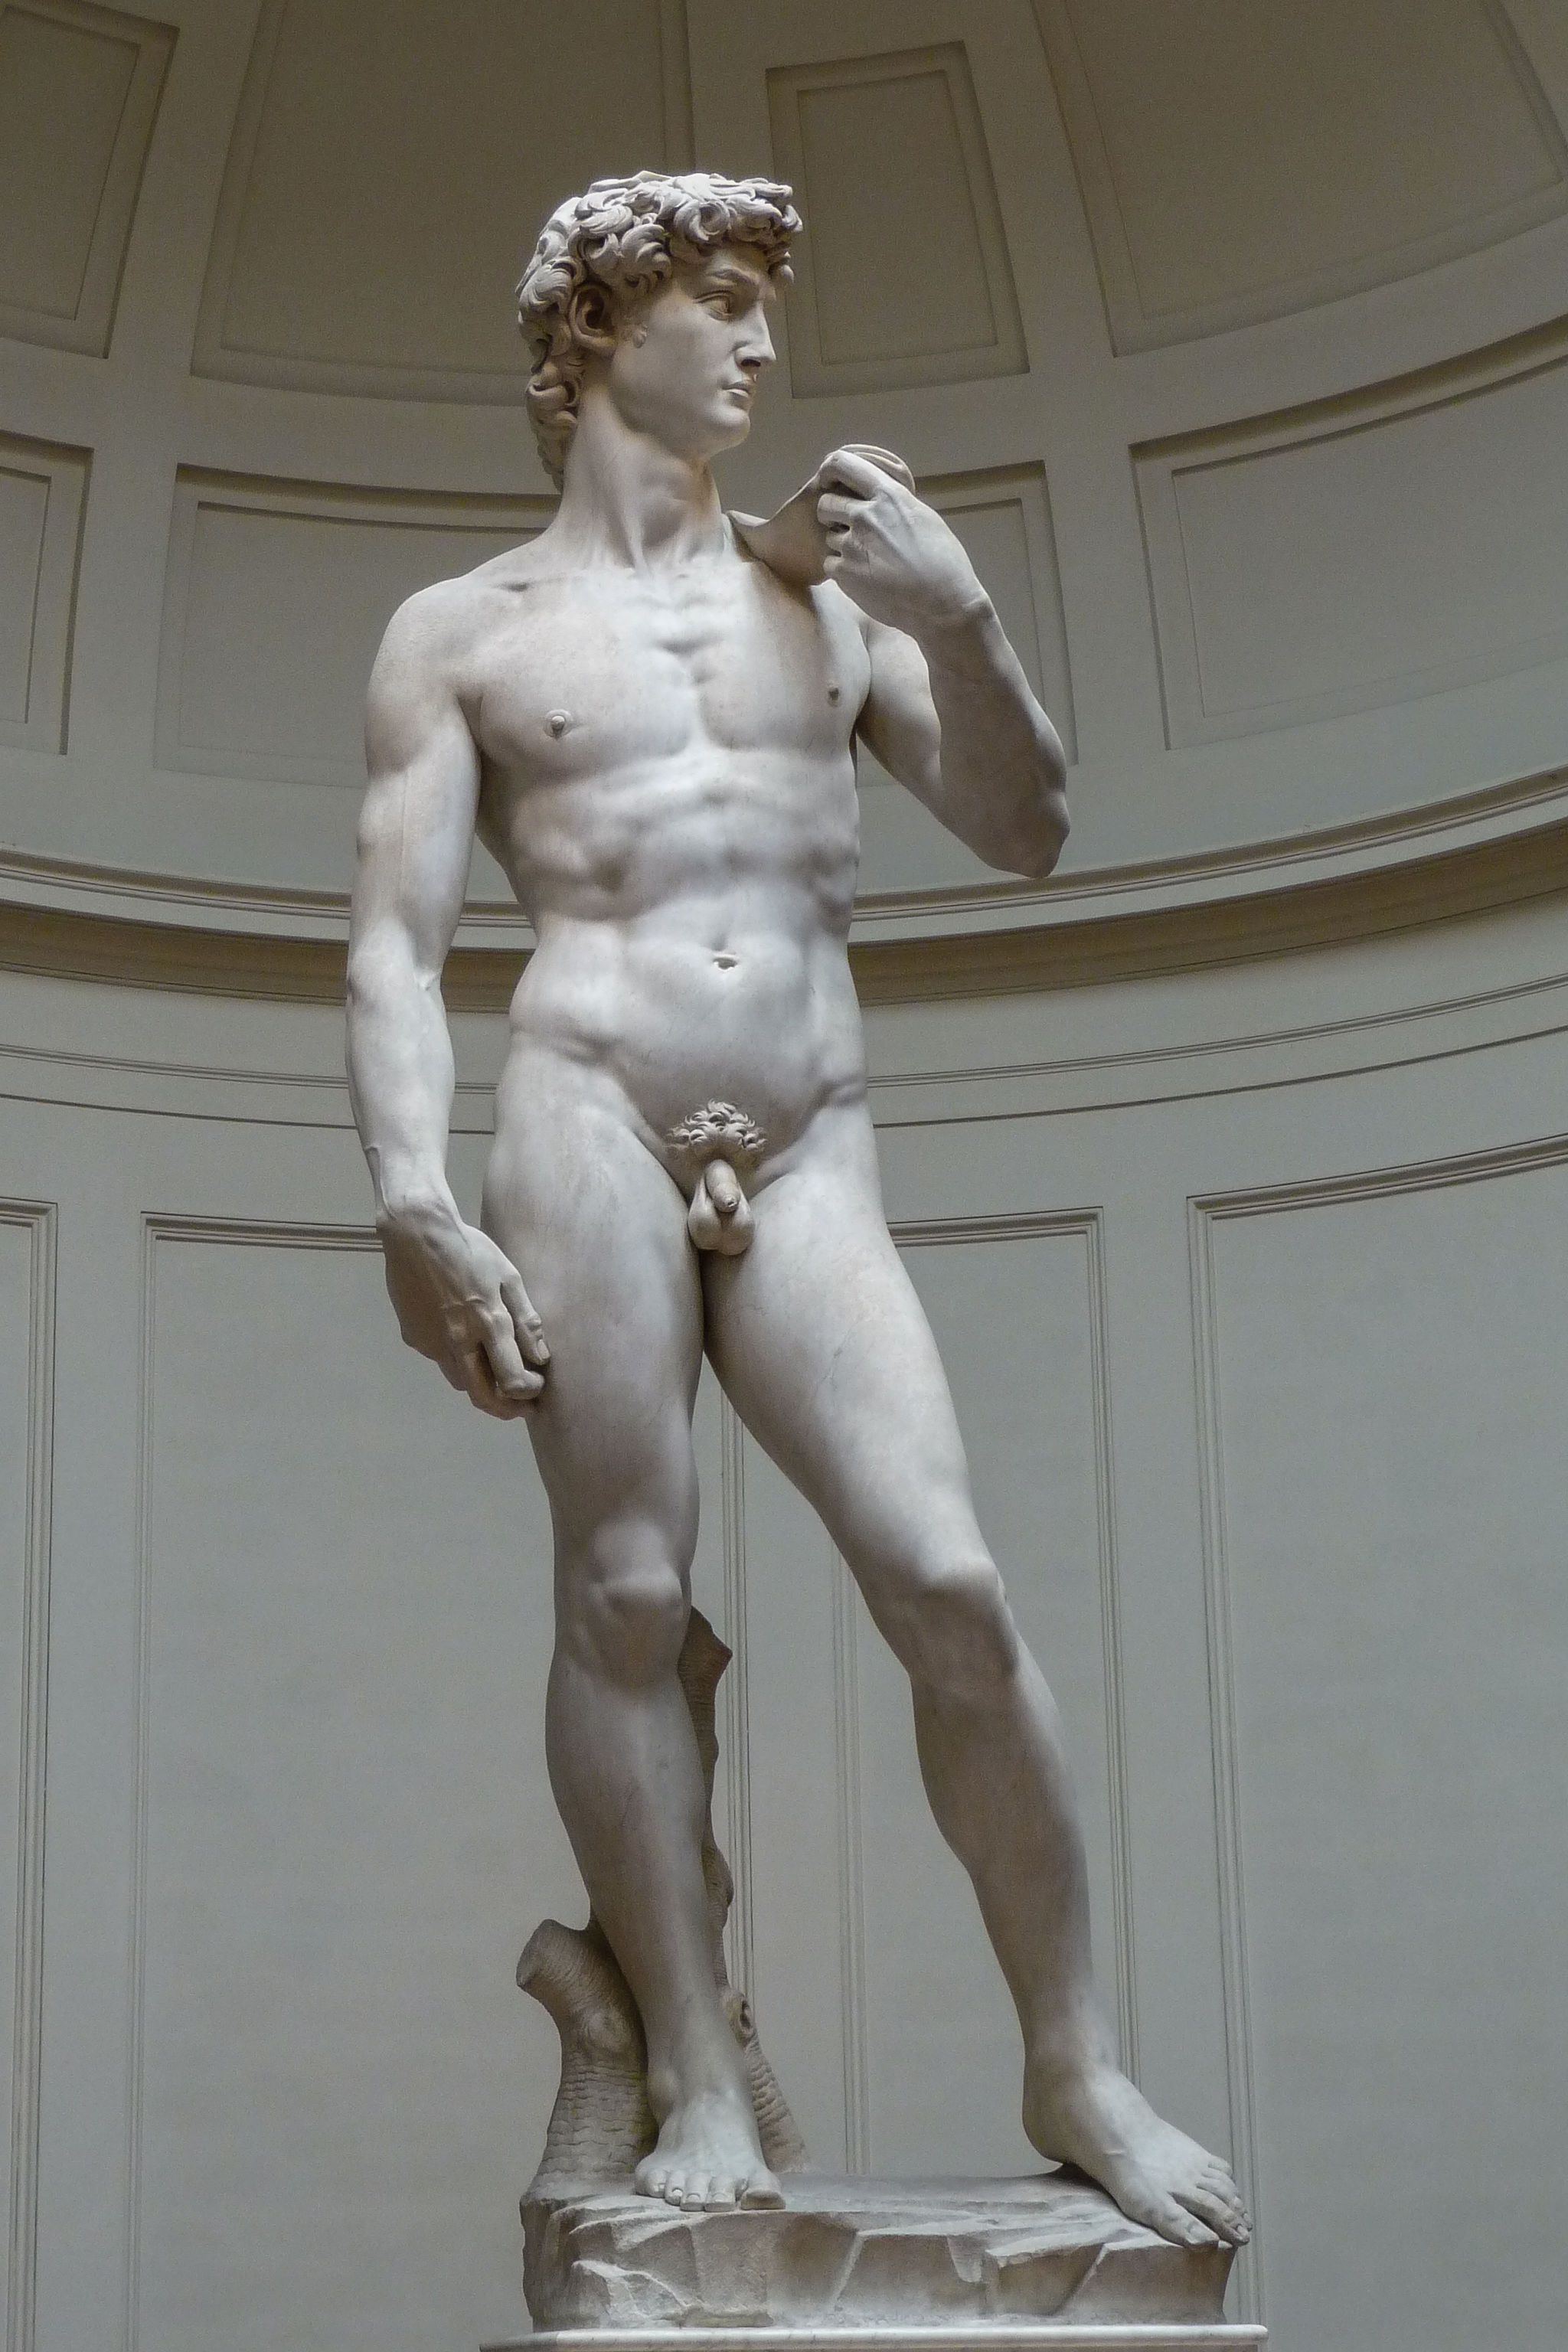
\includegraphics[width=0.30\textwidth]{figures/michelangelo_david}} \\
\onslide<3>{\LARGE{readymades}} &  & \onslide<3>{\LARGE{custommades}}
\end{tabular}
\end{center}

\vfill
\onslide<3>{
\TINY{\url{https://commons.wikimedia.org/wiki/File:Duchamp_Fountaine.jpg}}\\
\TINY{\url{https://commons.wikimedia.org/wiki/File:\%27David\%27_by_Michelangelo_JBU0001.JPG}}}

\end{frame}
%%%%%%%%%%%%%%%%%%%%%%%%%%
\begin{frame}

A few notes on my teaching:
\begin{itemize}
\item Anti-status quo bias
\pause
\item Anti-formality bias (formality is important, but just not right now)
\pause
\item Very brief, more information in Ch. 3 of \href{https://www.bitbybitbook.com/en/1st-ed/asking-questions/}{\textit{Bit by Bit}}
\end{itemize}

\end{frame}
%%%%%%%%%%%%%%%%%%%%%%%%%
\begin{frame}

We need surveys even in the digital age.

\end{frame}
%%%%%%%%%%%%%%%%%%%%%%%%%%%%%
\begin{frame}

We need surveys \sout{even} especially in the digital age.

\end{frame}
%%%%%%%%%%%%%%%%%%%%%%%%%%%%%
\begin{frame}

We will always need to ask
\begin{itemize}
\item limitations of big data (fubu vs.\ nufu-nubu)
\pause
\item internal states vs. external states
\pause
\item inaccessibility of big data
\end{itemize}

\pause
\vfill
But how we are going to ask is going to change
\end{frame}
%%%%%%%%%%%%%%%%%%%%%%%%%%%
\begin{frame}

\begin{center}
\begin{tabular}{ l c c}
           & Sampling& Interviews \\
\hline
1st era & Area probability & Face-to-face \\
\pause
2nd era & Random digital dial probability & Telephone \\
\pause
3rd era & \pause Non-probability & Computer-administered  \\
\end{tabular}
\end{center}

\end{frame}
%%%%%%%%%%%%%%%%%%%%%%%%%%%
\begin{frame}

\begin{center}
\small{
\begin{tabular}{ l c c c}
           & Sampling & Interviews & Data environment\\
\hline
1st era & Area probability & Face-to-face & Stand-alone \\
2nd era & \parbox[t]{3cm}{\centering Random digital dial\\probability} & Telephone & Stand-alone \\
3rd era & Non-probability & Computer-administered  & Linked \\
\end{tabular}
}
\end{center}

\end{frame}
%%%%%%%%%%%%%%%%%%%%%%%%%%%
\begin{frame}

\begin{center}
\small{
\begin{tabular}{ l c c c}
           & Sampling & Interviews & Data environment\\
\hline
1st era & Area probability & Face-to-face & Stand-alone \\
2nd era & \parbox[t]{3cm}{\centering Random digital dial\\probability} & Telephone & Stand-alone \\
\textcolor{blue}{3rd era} & \textcolor{blue}{Non-probability} & \textcolor{blue}{Computer-administered}  & \textcolor{blue}{Linked} \\
\end{tabular}
}
\end{center}

\end{frame}
%%%%%%%%%%%%%%%%%%%%%%%%%%%
\begin{frame}

\begin{center}
Total survey error framework
\end{center}

\end{frame}
%%%%%%%%%%%%%%%%
\begin{frame}
\frametitle{Total survey error framework}

Insight 1: Errors can come from bias and variance\\
\pause
\begin{center}
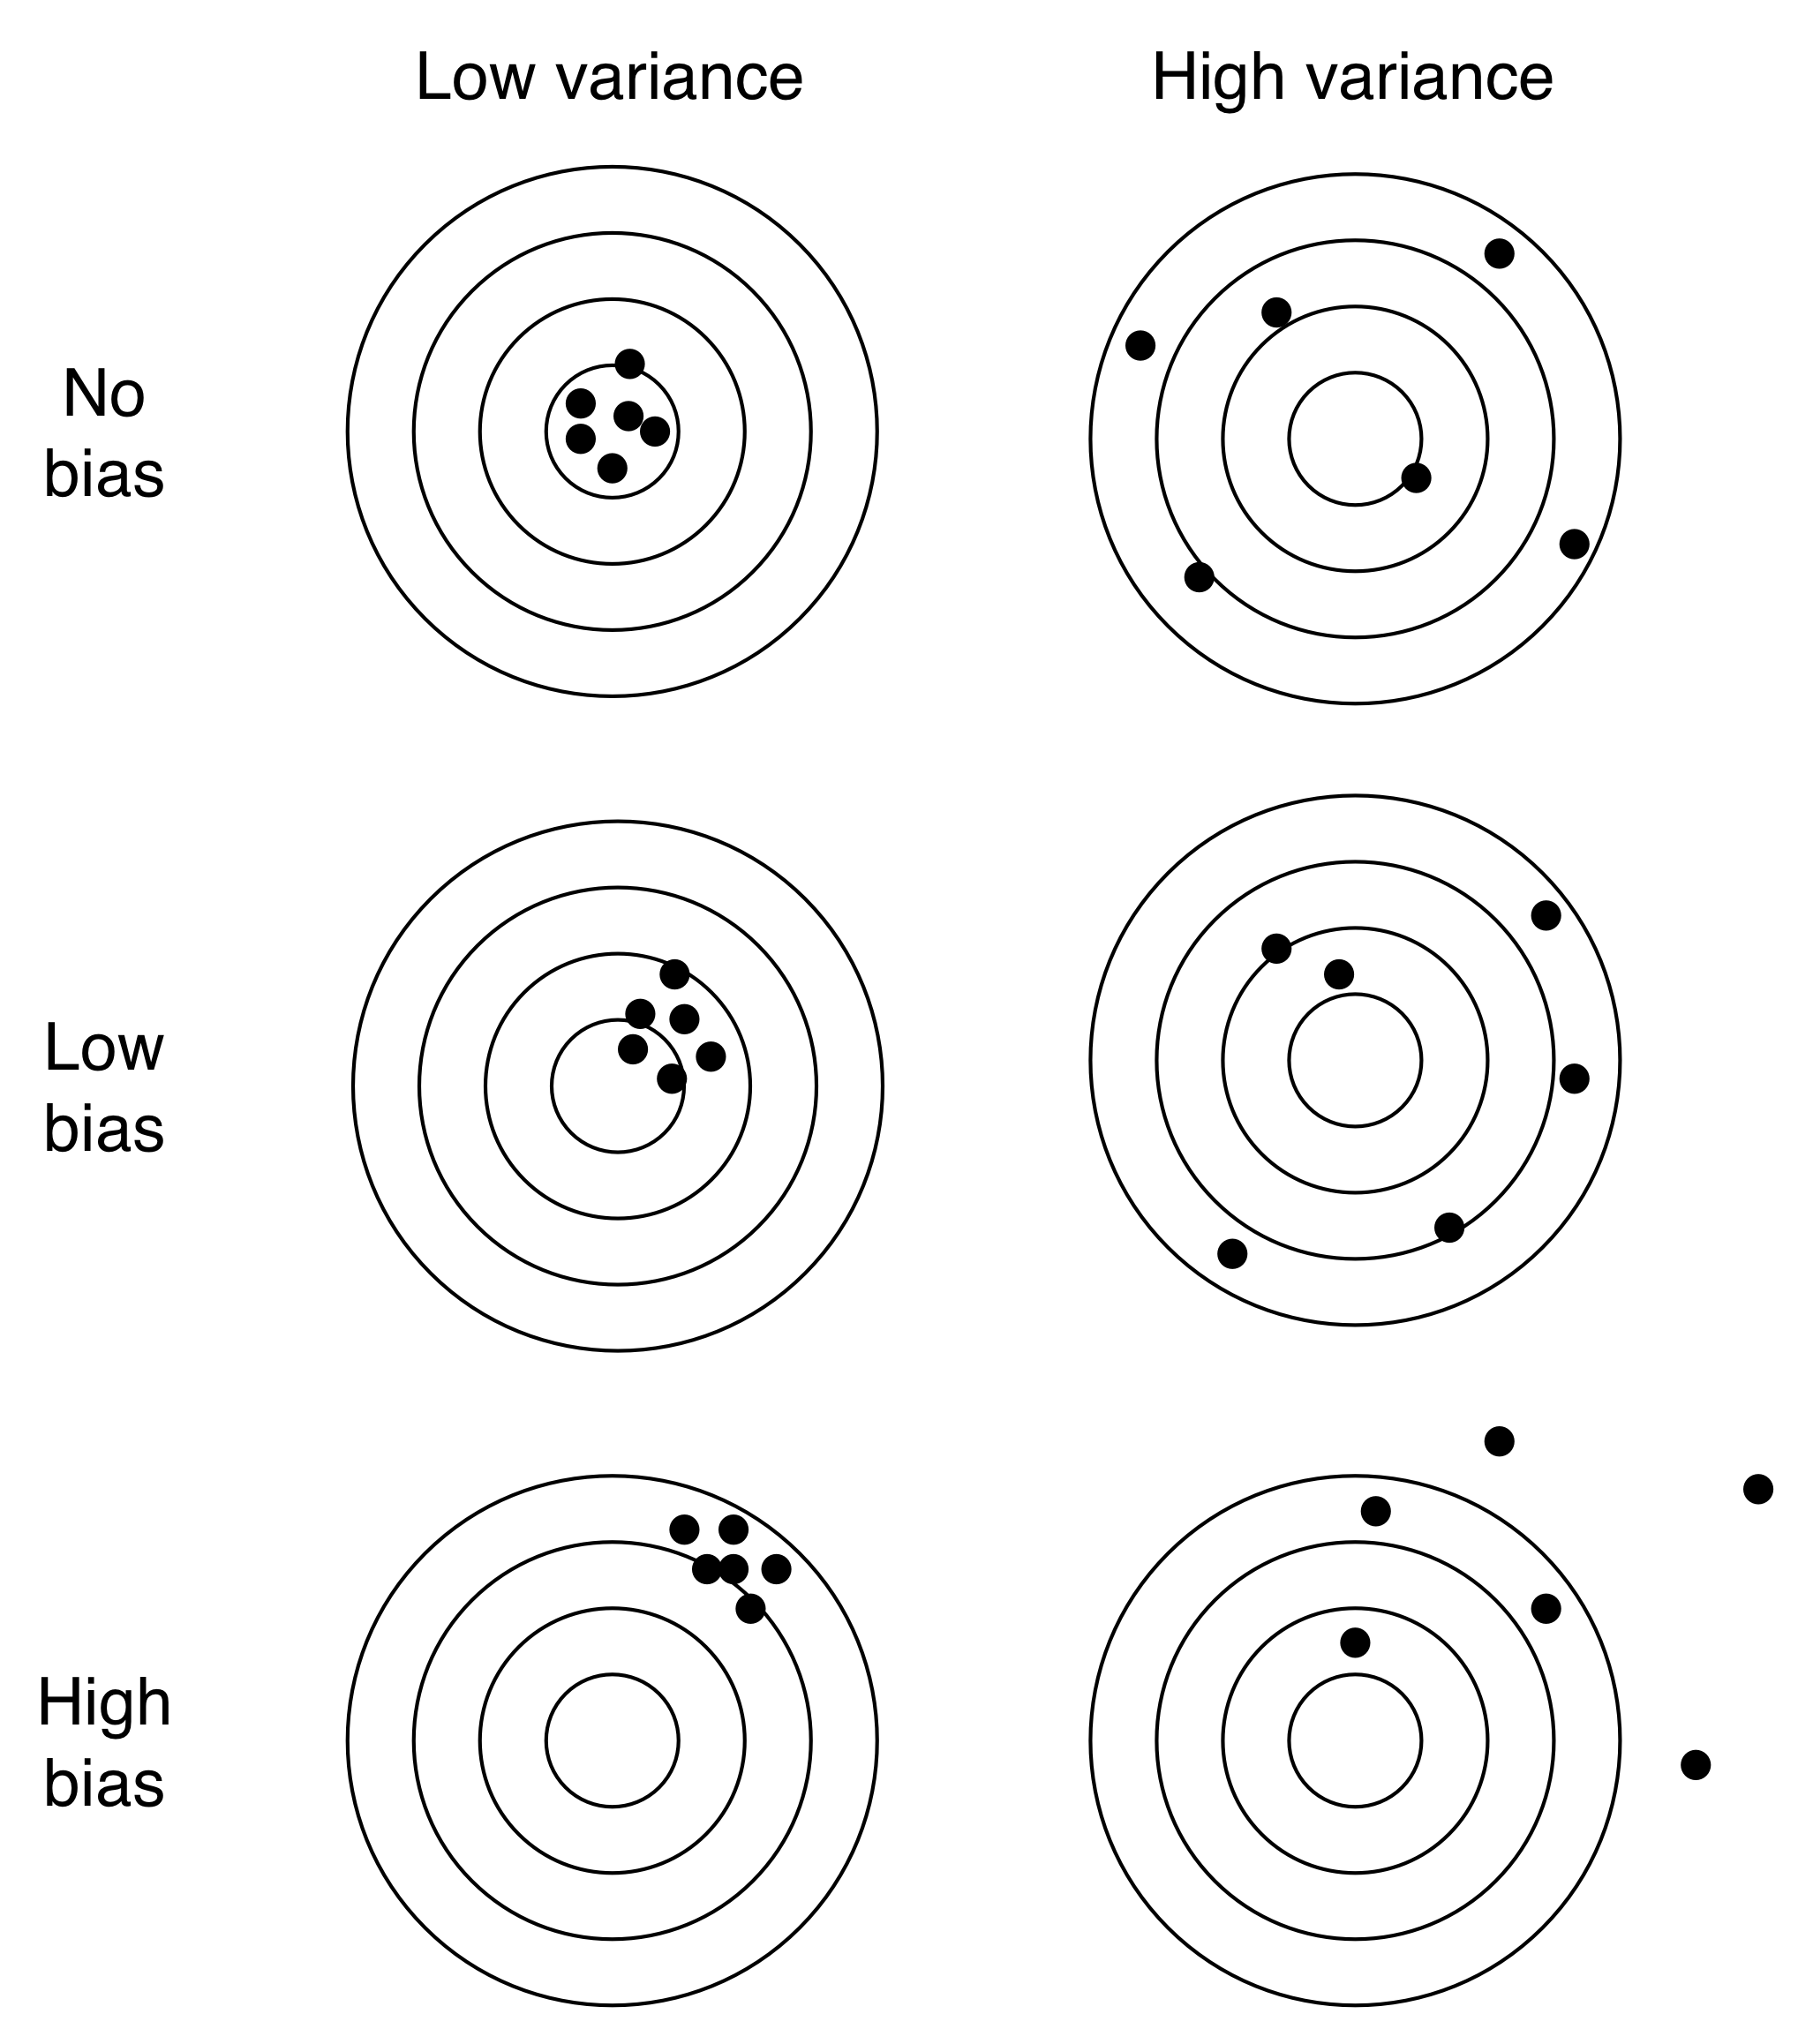
\includegraphics[height=0.6\textheight]{figures/bitbybit3-1_bias-variance}
\end{center}

\end{frame}
%%%%%%%%%%%%%%%%
\begin{frame}
\frametitle{Total survey error framework}

Insight 2: Total survey error = measurement error + representation error \\ 
\pause
\begin{center}
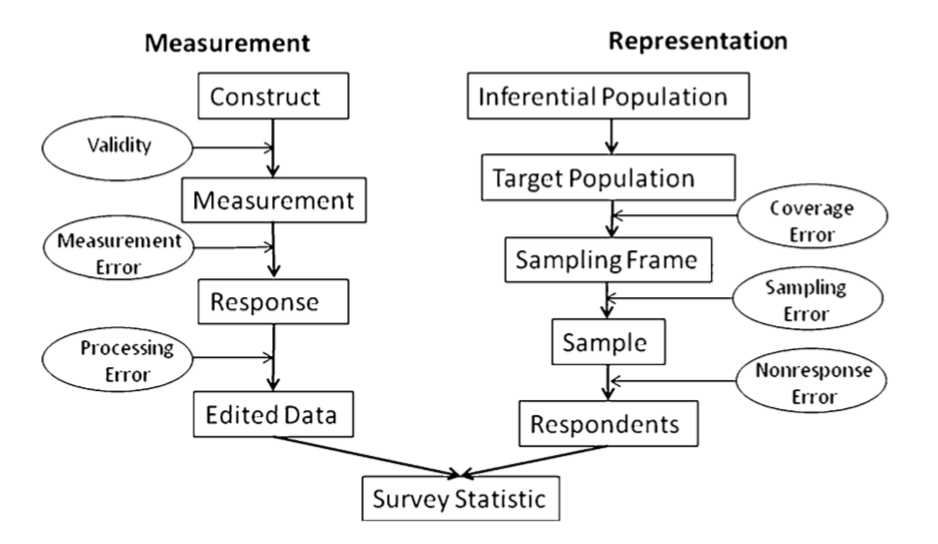
\includegraphics[width=0.6\textwidth]{figures/groves_total_2010_fig3}
\end{center}

\vfill
\small{\href{https://dx.doi.org/10.1093/poq/nfq065}{Groves and Lyberg 2010, Fig 3}}

\end{frame}
%%%%%%%%%%%%%%%%%%%%%%%%%%%
\begin{frame}
\frametitle{Case study of total survey error framework}

\begin{center}
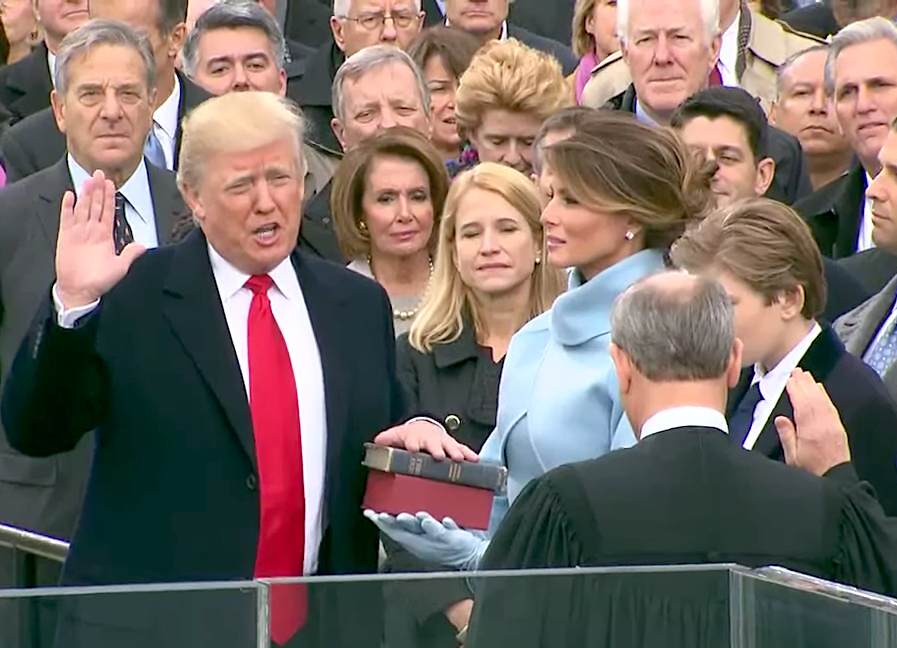
\includegraphics[width=0.6\textwidth]{figures/trump_oath}
\end{center}

\vfill
\tiny{\textcolor{blue}{\url{https://commons.wikimedia.org/wiki/File:Donald_Trump_taking_his_Oath_of_Office.png}}}

\end{frame}
%%%%%%%%%%%%%%%%%%%%%%%%%%
\begin{frame}
\frametitle{Case study of total survey error framework}

\begin{center}
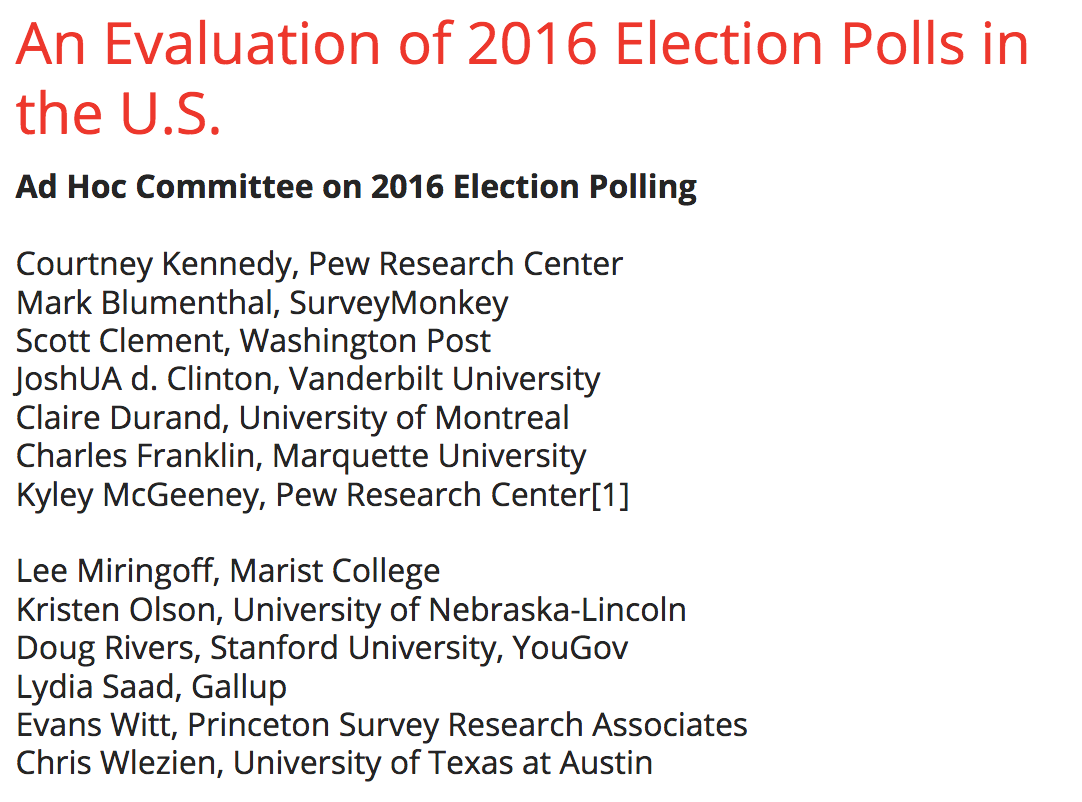
\includegraphics[width=0.5\textwidth]{figures/aapor_2016_election_evaluation}
\end{center}

\vfill
\tiny{\url{http://www.aapor.org/Education-Resources/Reports/An-Evaluation-of-2016-Election-Polls-in-the-U-S.aspx}}

\end{frame}
%%%%%%%%%%%%%%%%%%%%%%%%%%%
\begin{frame}
\frametitle{Case study of total survey error framework}

\begin{itemize}
\item National polls were generally correct and accurate by historical standards.
\pause
\item State-level polls showed a competitive, uncertain contest  . . . 
\pause
\item  . . . but clearly under-estimated Trump's support in the Upper Midwest.
\end{itemize}

\end{frame}
%%%%%%%%%%%%%%%%%%%%%%%%%%%%
\begin{frame}
\frametitle{Case study of total survey error framework}

``There are a number of reasons as to why polls under-estimated support for Trump. The explanations for which we found the most evidence are:''
\begin{itemize}
\item ``Real change in vote preference during the final week or so of the campaign''
\pause
\item ``Adjusting for over-representation of college graduates was critical, but many polls did not do it''
\pause
\item ``Some Trump voters who participated in pre-election polls did not reveal themselves as Trump voters until after the election, and they outnumbered late-revealing Clinton voters''
\end{itemize}

\vfill

Full report: \url{http://www.aapor.org/Education-Resources/Reports/An-Evaluation-of-2016-Election-Polls-in-the-U-S.aspx}

\end{frame}
%%%%%%%%%%%%%%%%%%%%%%%%%%%%%%
\begin{frame}
\frametitle{Conclusion}

Wrapping up:
\pause
\begin{itemize}
\item We need surveys especially in the digital age.
\pause
\item Total survey error framework 1st key insight: errors can be caused by bias and variance
\pause
\item Total survey error framework 2nd key insight: errors can be related to representation and measurement
\pause
\item Total survey error framework also helps us think about how digital age can create new opportunities (who to ask and how to ask)
\pause 
\item To learn more: \href{https://www.amazon.com/Survey-Methodology-Robert-M-Groves/dp/0470465468}{Groves et al (2009)}
\end{itemize}

\end{frame}
%%%%%%%%%%%%%%%%%%%%%%%%%%%%%%
\frame{\titlepage}
%%%%%%%%%%%%%%%%%%%%%%%%%%%%%%

\end{document}
